\chapter{Многомодовые когерентные состояния и их интерференция}  \label{ch:ch4}
\section{Квантовое описание когерентного состояния} \label{sec:ch4/sec1}

Термин \textit{когерентное состояние} был введен Р. Дж. Глаубером. в 1963 г. Оно не совсем соотносится с классическим термином когерентность, но имеет отношение к специальному типу чистых квантово-механических состояний светового поля, соответствующего одиночной моде резонатора. Когерентное состояние определяется, как суперпозиция Фоковских состояний, то есть состояний числа фотонов. 


\begin{equation}
	\begin{aligned}
		|\alpha \rangle = \sum_{n=0}^\infty   |  \rangle,
	\end{aligned}
\end{equation}

Комплексное число $ \alpha $	определяется среднее число фотонов, которое равно квадрату модуля, и фазой когерентного состояния. Из выражения видно, что вероятность нахождения n фотонов в когерентном состоянии определяется, как показано в уравнении. 

\begin{equation}
	\begin{aligned}
		|\alpha \rangle = \sum_{n=0}^\infty   |  \rangle,
	\end{aligned}
\end{equation}

где - это среднее число фотонов. Видно, что когерентное состояние подчиняется распределению Пуассона. Когерентное состояние имеет свойства близкие классическим состояниям света. Отдельный случай когерентного состояния - это когда =0. Оно называется вакуумным состоянием с нулевым числом фотонов. Однако, в таком случае все равно наблюдаются квантовые флуктуации электрического и магнитного полей, которые иногда называют вакуумным шумом. 


%	\pagebreak

%%%%%%%%%%%%%%%%%%%%%%%%%%%%%%%%%%%%%%%%%%%%%%%%%%%%%%%%%%%%%%%%%%%%%%%%%%%%%%%%%%%%%%%%%%%%%%%%%%%%%%%%%%%%%%%%%
\section{Когерентные состояния после прохождения светоделителя} \label{ch:ch4/sect2}
 

 \begin{figure}[ht]
  \centering
  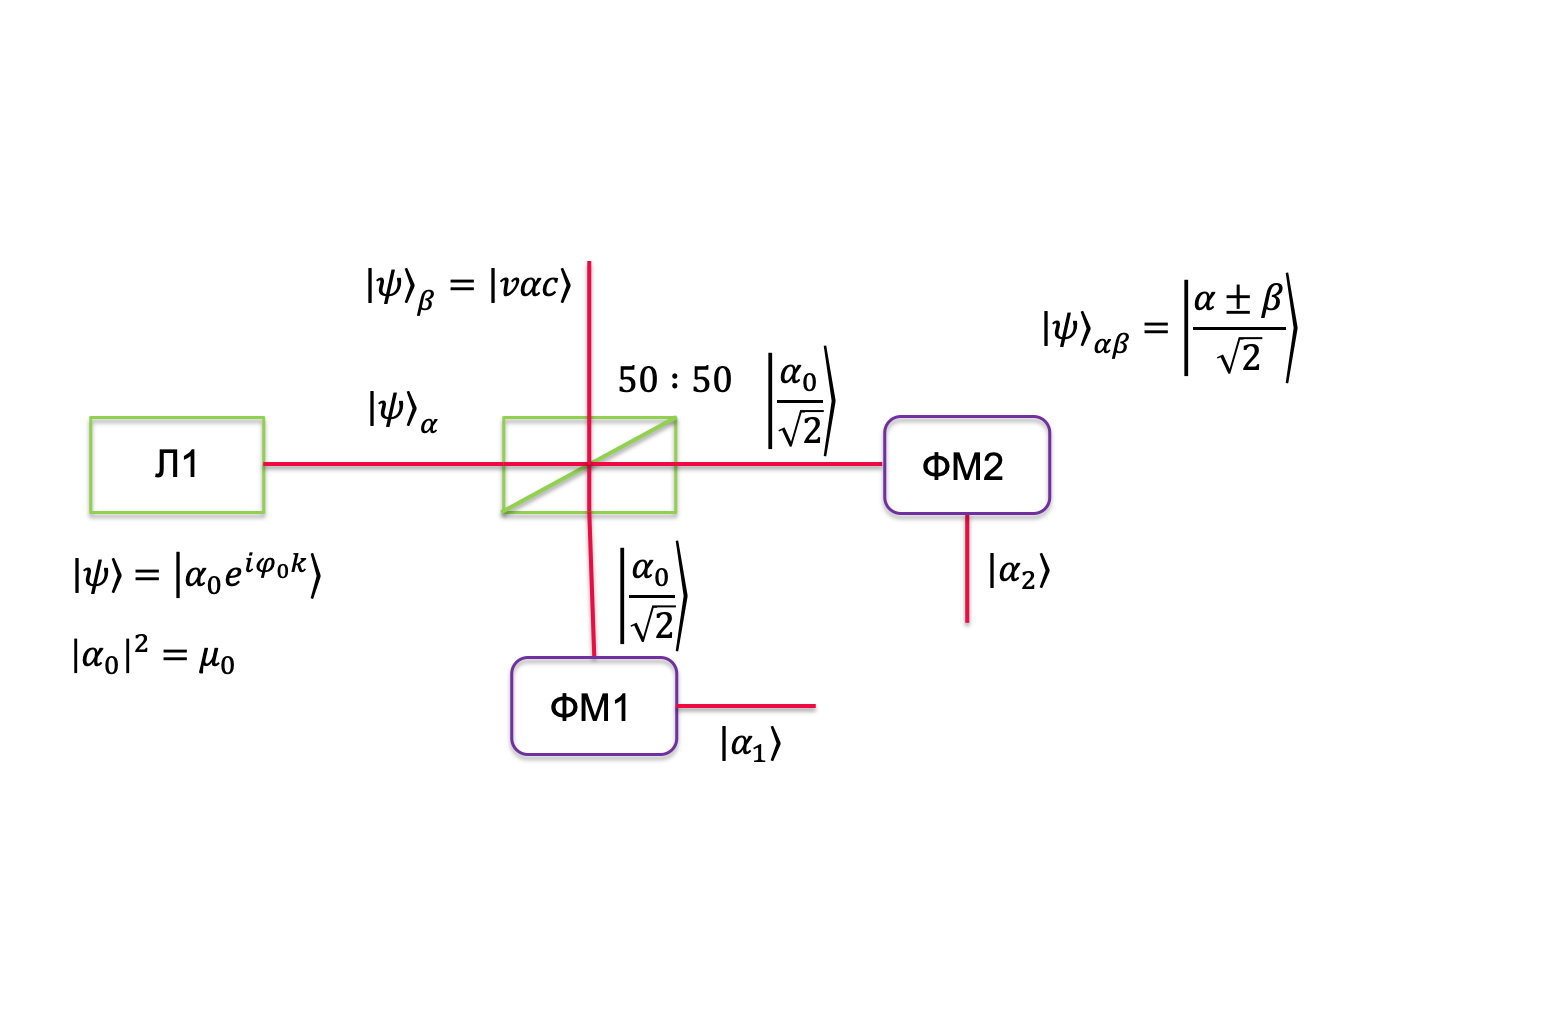
\includegraphics[scale=0.8]{Coherent_states_beamsplitting.png}
  \caption{Принципиальная схема наблюдения динамики когерентных состояний}
  \label{fig:Coherent_states_beamsplitting}
\end{figure}

\pagebreak

%%%%%%%%%%%%%%%%%%%%%%%%%%%%%%%%%%%%%%%%%%%%%%%%%%%%%%%%%%%%%%%%%%%%%%%%%%%%%%%%%%%%%%%%%%%%%%%%%%%%%%%%%%%%%%%%%
\section{Когерентные состояния после модуляции} \label{ch:ch4/sect3}

Отличительно особенностью систем квантовой коммуникации на боковых частотах модулированного излучения является генерация многомодовых когерентных состояний на разных оптических модах, зависящих от частоты модулирующего сигнала. 

 \begin{figure}[ht]
  \centering
  \includegraphics[scale=0.5]{Modes_rus.pdf}
  \caption{Принципиальная схема генерации боковых частот}
  \label{fig:multimodes}
\end{figure}

\pagebreak

%%%%%%%%%%%%%%%%%%%%%%%%%%%%%%%%%%%%%%%%%%%%%%%%%%%%%%%%%%%%%%%%%%%%%%%%%%%%%%%%%%%%%%%%%%%%%%%%%%%%%%%%%%%%%%%%%
\section{Результат интерференции когерентных состояний после модуляции} \label{ch:ch4/sect4}

\begin{figure}[ht]
 \centering
  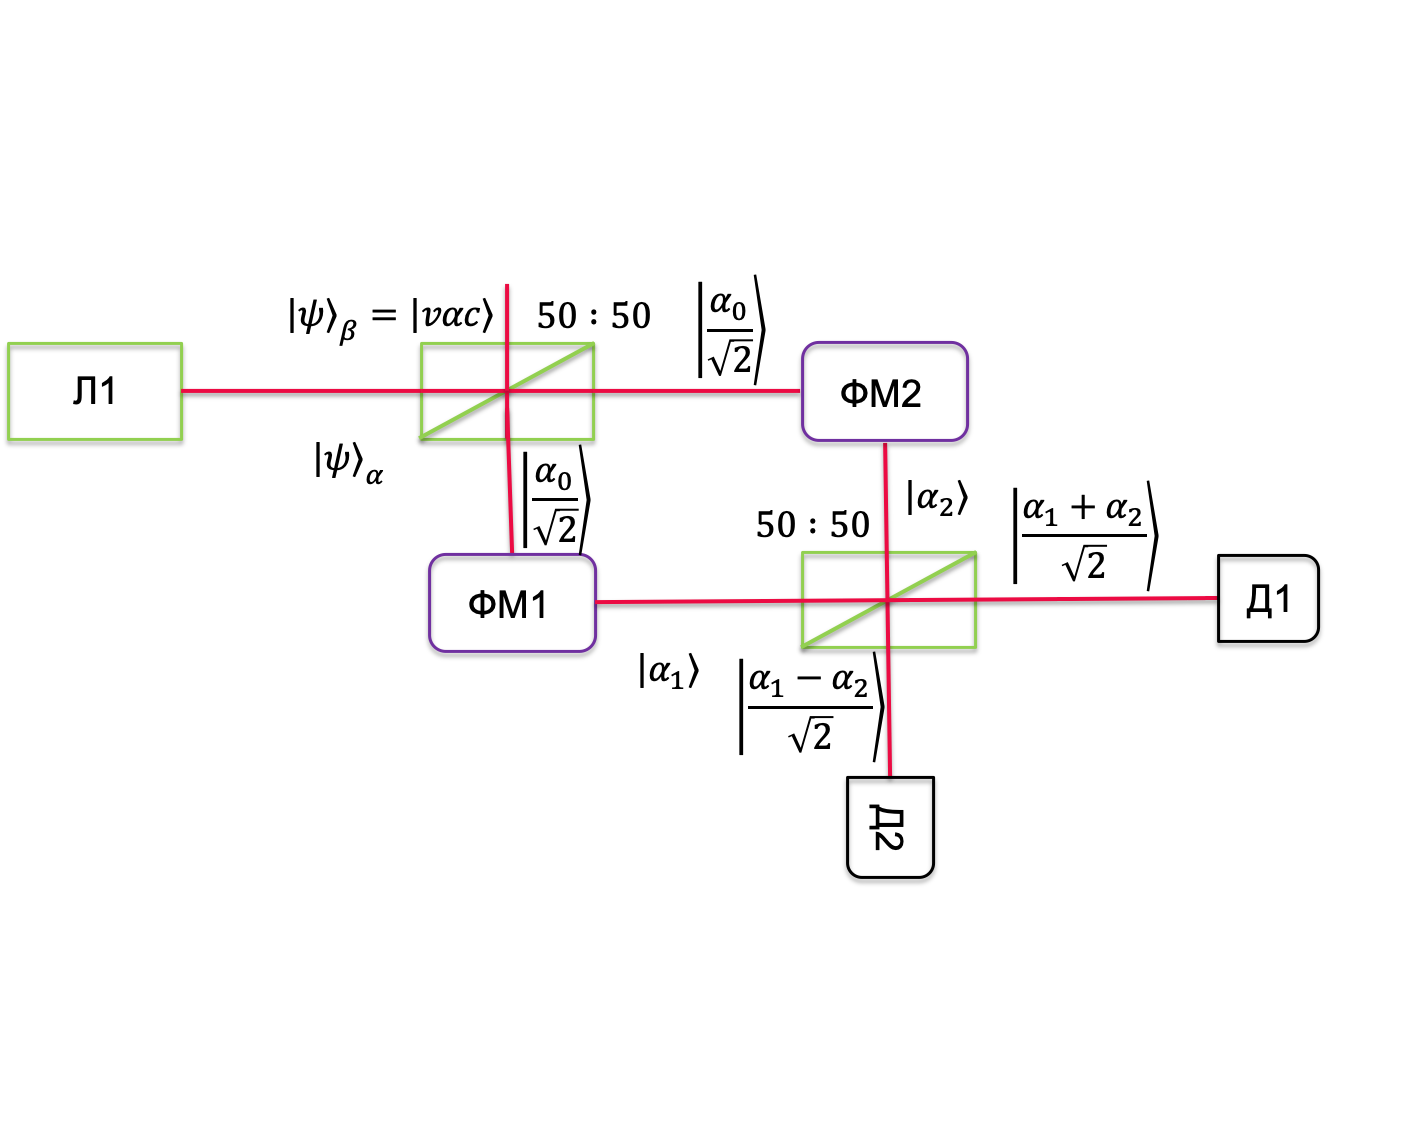
\includegraphics[scale=0.5]{Coherent_state_beamsplitting2.png}
  \caption{Принципиальная схема наблюдения динамики когерентных состояний}
  \label{fig:Coherent_states_beamsplitting2}
\end{figure}

\pagebreak

%%%%%%%%%%%%%%%%%%%%%%%%%%%%%%%%%%%%%%%%%%%%%%%%%%%%%%%%%%%%%%%%%%%%%%%%%%%%%%%%%%%%%%%%%%%%%%%%%%%%%%%%%%%%%%%%%
\section{Зависимость результата интерференции от разности фаз когерентных состояний} \label{ch:ch4/sect5}


\begin{figure}[ht]
 \centering
  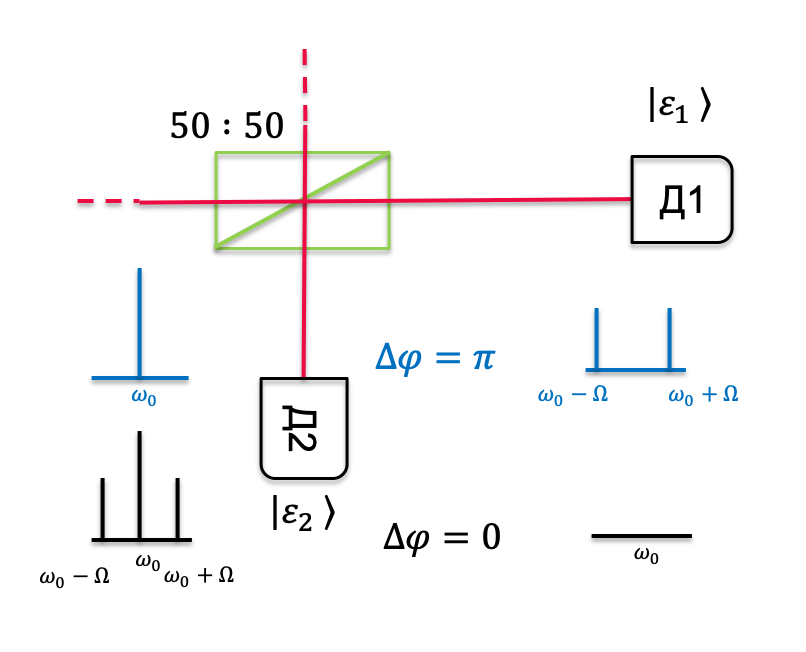
\includegraphics[scale=0.9]{Interference_result.png}
  \caption{Принципиальная схема наблюдения результата интерференции когерентных состояний}
  \label{fig:Interference_result}
\end{figure}

\pagebreak

%%%%%%%%%%%%%%%%%%%%%%%%%%%%%%%%%%%%%%%%%%%%%%%%%%%%%%%%%%%%%%%%%%%%%%%%%%%%%%%%%%%%%%%%%%%%%%%%%%%%%%%%%%%%%%%%%
\section{Протокол системы квантовой рассылки ключа, устойчивый к атакам на измерительное оборудование} \label{ch:ch4/sect6}

\begin{figure}[ht]
 \centering
  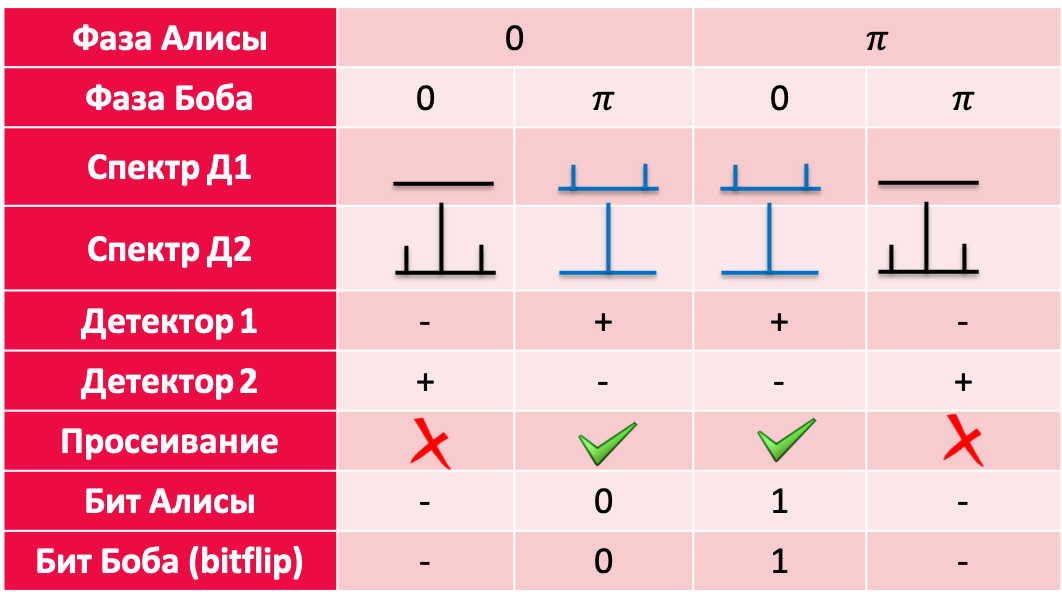
\includegraphics[scale=0.9]{Protocol.png}
  \caption{Протокол}
  \label{fig:Protocol}
\end{figure}


\pagebreak

%%%%%%%%%%%%%%%%%%%%%%%%%%%%%%%%%%%%%%%%%%%%%%%%%%%%%%%%%%%%%%%%%%%%%%%%%%%%%%%%%%%%%%%%%%%%%%%%%%%%%%%%%%%%%%%%%
\section{Выводы по главе} \label{ch:ch4/sect7}


В \ref{ch:ch4} главе показано, что метод квантовой коммуникации на боковых частотах позволяет реализовывать протокол, устойчивый к контролю нелегитимным пользователем измерительного оборудования. 
 
\pagebreak

